\subsection{Introduction to Differential Equations}



\frame{
Consider the equation 
\begin{equation}
\frac{dy}{dt} = 1 - e^{-t}
\label{eq_7-1}
\end{equation}
%\begin{figure}
%\begin{center}
%\includegraphics[width=70mm]{fig/ch-6/eq_6-1.png}
%\end{center}
%\end{figure}
\begin{block}{}
\begin{itemize}
\item It is a differential equation because it involves the derivative $dy / dt$ of the "unknown function" $y = y(t)$. 
\vspace{0.3cm}
\item Only the independent variable t appears on the right side of equation (6.1): hence a solution is an antiderivative of $1 - e^{-t}$.
\end{itemize}
\end{block}
}

\frame{
The rules of integration can be used to find $y(t)$ :
\begin{equation}
y(t) = t + e^{-t} + C,
\label{eq_7-2}
\end{equation}
%\begin{figure}
%\begin{center}
%\includegraphics[width=70mm]{fig/ch-6/eq_6-2.png}
%\end{center}
%\end{figure}
where $C$ is the constant of integration. 
\vspace{0.5cm}
\begin{itemize}
\item All the functions in (2 ) are solutions of (1) because they satisfy the requirement that $y' (t) = 1 - e^{-t}$. 
\vspace{0.3cm}
\item They form the family of curves in Figure 6.2.
\end{itemize}
}


\frame{
\begin{figure}
\begin{center}
%\includegraphics[width=80mm]{fig/ch-6/fig_6-2.png}
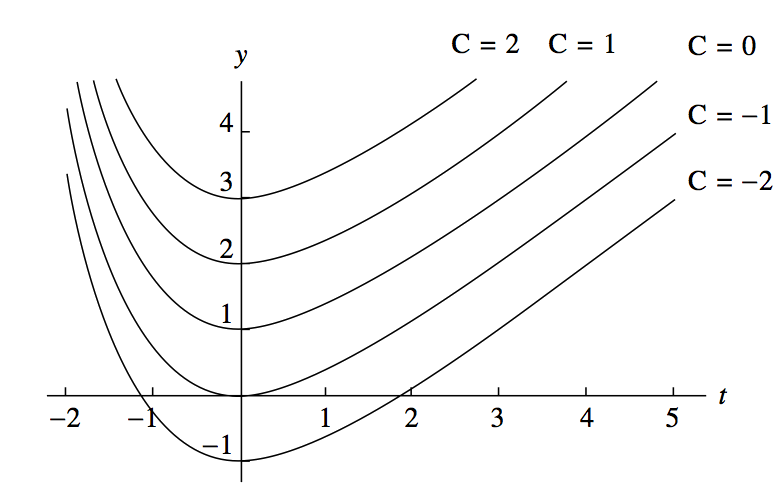
\includegraphics[width=80mm]{chap-6/fig_9-2.png}
%\label{Figure 9.2}
\end{center}
\end{figure}
When this is translated into a mathematical model,  
the result is an equation involving the rate of change of the unknown function and the independent and/or dependent variable. 
}

\frame{
\begin{itemize}
\item Integration was the technique used to find the explicit formula for the functions in (\ref{eq_7-2}), and Figure 6.2 emphasizes that there is one degree of freedom involved in the solution, that is, the constant of integration $C$. 
\item By varying the value of $C$, we "move the solution curve" up or down, and a particular curve can be found that will pass through any desired point. 
\vspace{0.5cm}
\item The secrets of the world are seldom observed as explicit formulas. 
\item Instead, we usually measure {\Large how a change in one variable affects another variable}. 
\end{itemize}
}


\frame{
\frametitle{Consider the temperature $y(t)$ of a cooling object.} 
\begin{itemize}
\item It might be conjectured that the rate of change of the temperature of the body is related to the temperature difference between its temperature and that of the surrounding medium. 
\item Experimental evidence verifies this conjecture. 
\item Newton's law of cooling asserts that the rate of change is  directly proportional to the difference in these temperatures. 
\end{itemize}
}

\frame{
If A is the temperature of the surrounding medium and $y(t)$ is the temperature of the body at time $t$, then 
\begin{equation}
\frac{dy}{dt} = -k (y-A)
\end{equation}
%\begin{figure}
%\begin{center}
%\includegraphics[width=60mm]{fig/ch-6/eq_6-3.png}
%\end{center}
%\end{figure}
where $k$ is a positive constant. \\
The negative sign is required because $dy \slash dt$ will be negative when the temperature of the body is greater than the temperature of the medium. 
}

\frame{
If the temperature of the object is known at time $t = 0$, 
we call this an initial condition and include this information in the statement of the problem. \\
Usually, we are asked to solve 
\begin{equation}
\frac{dy}{dt} =  -k (y - A) \ \ with \ \ y(0) = y_0
\end{equation}
%\begin{figure}
%\begin{center}
%\includegraphics[width=80mm]{fig/ch-6/eq_6-4.png}
%\end{center}
%\end{figure}
The technique of separation of variables can be used to find the solution
\begin{equation}
y = A + \left( y_0 - A \right) e^{-kt}
\end{equation}
%\begin{figure}
%\begin{center}
%\includegraphics[width=80mm]{fig/ch-6/eq_6-5.png}
%\end{center}
%\end{figure}
}

\frame{
\begin{itemize}
\item For each choice of $y_0$, the solution curve will be different, and there is no simple way to move one curve around to get another one. 
\item The initial value is a point where the desired solution is "nailed down." 
\item Several solution curves are shown in the following figure\footnote{Figure 6.3 in the textbook}, and it can be observed that as $t$ gets large the temperature of the object approaches room temperature. 
\item If $y_0 < A$, the body is warming instead of cooling. 
\end{itemize}

\begin{figure}
\begin{center}
%\includegraphics[width=100mm]{fig/ch-6/fig_6-3.png}
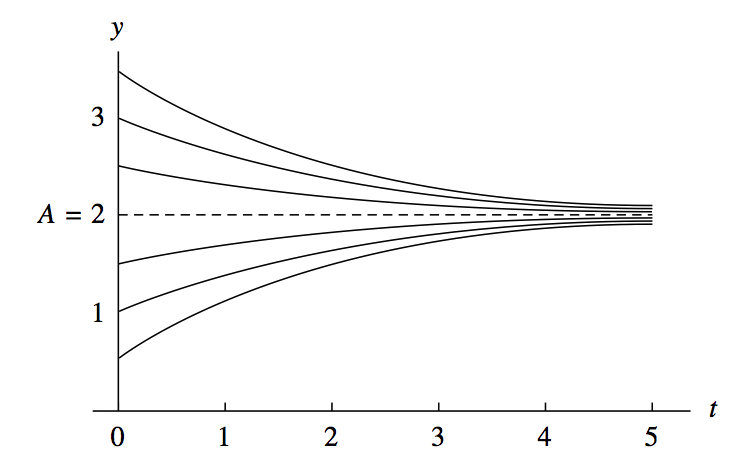
\includegraphics[width=60mm]{chap-6/fig_9-3.png}
\end{center}
\end{figure}
}



\frame{
\frametitle{ Initial Value Problem}
\begin{block}{Definition 6.1. A solution to the initial value problem (I.V.P.)}
\begin{equation*}
y′ = f (t, y) \ \ \ with \ \ \ y(t_0) = y_0
\end{equation*}
on an interval $[t_0, b]$ is a differentiable function $y = y(t)$ such that
\begin{equation*}
y(t_0) = y_0 \ \ \ and \ \ \ y′ = f (t, y(t)) \ \ \ for \ all \ t \in [t_0, b] 
\end{equation*}
Notice that the solution curve $y = y(t)$ must pass through the initial point $(t_0, y_0)$. 
\end{block}
%\begin{figure}
%\begin{center}
%\includegraphics[width=110mm]{fig/ch-6/def_6-1.png}
%\end{center}
%\end{figure}
}

\frame{
\frametitle{Geometric Interpretation}
\begin{itemize}
\item At each point $(t, y)$ in the rectangular region $R = \{( t, y) : a \le t \le b, c \le y \le d\}$, 
the slope of a solution curve $y = y(t)$ can be found using the implicit formula $m = l(t, y(t))$. 
\vspace{0.5cm}
\item Hence the values $m_{i,j} = f (t_i, y_j)$ can be computed throughout the rectangle, 
and each value $m_{i,j}$ represents the slope of the line tangent to a solution curve that passes through the point $(t_i,y_j)$. 
\end{itemize}
}

\frame{
A slope field or direction field is a graph that indicates the slopes $\{m_{i,j}\}$ over the region.  \\
It can be used to visualize how a solution curve "fits" the slope constraint. 
\begin{itemize}
\item To move along a solution curve, one must start at the initial point and check the slope field to determine in which direction to move. 
\item Then take a small step from $t_0$ to $t_0 + h$ horizontally and move the appropriate vertical distance $hf(t_0, y_0)$ so that the resulting displacement has the required slope. 
\item The next point on the solution curve is $(t_1, y_1)$. 
\item Repeat the process to continue your journey along the curve. 
\item Since a finite number of steps will be used, the method will produce an approximation to the solution. 
\end{itemize}
}

\frame{
\begin{block}{Example6.1.}
The slope field for $y′=(t-y)\slash 2$ over the rectangle $R = \{(t,y) : 0 \le t \le  5, 0 \le y \le 4\}$ is shown in the following figure\footnote{Figure 6.4 in textbook}. 
\end{block}
The solution curves with the following initial values are shown:
\begin{itemize}
\item For $y(0) = 1$, the solution is $y(t) = 3e^{-t\slash2} - 2 + t$.
\item For $y(0) = 4$, the solution is $y(t) = 6e^{-t\slash2} - 2 + t$.
\end{itemize}
%\begin{figure}
%\begin{center}
%\includegraphics[width=110mm]{fig/ch-6/ex_6-1.png}
%\end{center}
%\end{figure}
\begin{figure}
\begin{center}
%\includegraphics[width=80mm]{fig/ch-6/fig_6-4.png}
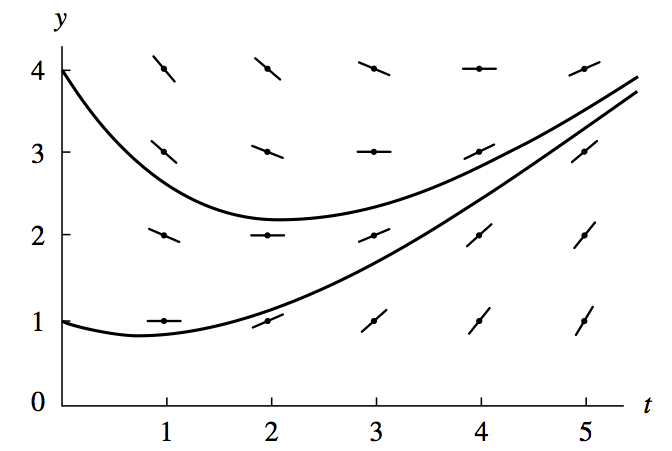
\includegraphics[width=60mm]{chap-6/fig_9-4.png}
\end{center}
\end{figure}
}

\frame{
\begin{block}{Definition 6.2.}
Given the rectangle $R = \{(t, y) : a \le t \le b, c \le y \le d \}$, 
assume that $f (t, y)$ is continuous on $R$.\\
The function $f$ is said to satisfy a {\Large Lipschitz condition} in the variable $y$ on $R$ provided that a constant $L > 0$ exists with the property that
\begin{equation*}
\left| f(t,y_1) - f(t,y_2)\right| \le L\left| y_1 - y_2 \right|
\end{equation*}
whenever $(t, y_1)$, $(t, y_2) \in R$. \\
The constant $L$ is called a {\Large Lipschitz constant} for $f$.
\end{block}
%\begin{figure}
%\begin{center}
%\includegraphics[width=110mm]{fig/ch-6/def_6-2.png}
%\end{center}
%\end{figure}
}

\frame{
\begin{block}{Theorem 6.1.}
Suppose that $f (t, y)$ is defined on the region $R$.  \\
If there exists a constant $L > 0$ so that
\begin{equation*}
\left| f_y (t, y) \right| \le L \ \ \ for \ \ all \ (t,y) \in R,
\end{equation*}
then $f$ satisfies a Lipschitz condition in the variable $y$ with Lipschitz constant $L$ over
the rectangle $R$.
\end{block}
Proof. \\
Fix $t$ and use the mean value theorem to get $c_1$ with $y_1 < c_1 < y_2$ so that
\begin{equation*}
\begin{array}{r l}
|f(t,y_1)- f(t,y_2)| & = |f_y(t,c_1)(y_1-y_2)| \\
& \\
& = | f_y (t , c_1 )|| y_1 - y_2 | \le L | y_1 - y_2 |.
\end{array}
\end{equation*}
%\begin{figure}
%\begin{center}
%\includegraphics[width=110mm]{fig/ch-6/theorem_6-1.png}
%\end{center}
%\end{figure}
%\begin{figure}
%\begin{center}
%\includegraphics[width=110mm]{fig/ch-6/theorem_6-1_proof.png}
%\end{center}
%\end{figure}
}

\frame{
\begin{block}{Theorem 6.2 (Existence and Uniqueness).}
\begin{itemize}
\item Assume that $f(t, y)$ is continuous in a region $R = \{( t, y) : t_0 \le t \le b, c \le y \le d\}$. 
\item If f satisfies a Lipschitz condition on $R$ in the variable $y$ and $(t_0, y_0) \in R$, then the initial value problem (6.6), $y' = f(t, y)$  with $y(t_0) = y_0$, has a unique solution $y = y(t)$ on some subinterval $t_0 \le t  \le t_0 + \delta$. 
\end{itemize}
\end{block}
}

\frame{
\begin{itemize}
\item Let us apply Theorems 6.1 and 6.2 to the function $f(t, y) = (t - y)/2$. 
\item The partial derivative is $f_y(t, y) = -1/2$. 
\item Hence $| f_y(t, y)| \le \frac{1}{2}$ and, according to Theorem 6.1, the Lipschitz constant is $L = \frac{1}1{2}$.
\item Therefore, by Theorem 6.2 the I.V.P. has a unique solution. 
\end{itemize}
%\begin{itemize}
%\item Sketches of the slope field and solution curves can be constructed by using the meshgrid and quiver commands in MATLAB. 
%\item The following M-file will generate a graph analogous to Figure 6.4. 
%\item In general, care must be taken to avoid points $(t, y)$ at which $y'$ is undefined. 
%\end{itemize}
}

%\frame{
%\begin{columns}
%\begin{column}{0.7\textwidth}
%\begin{figure}
%\begin{center}
%\includegraphics[width=80mm]{fig/ch-6/fig_6-4.png}
%\end{center}
%\end{figure}
%\end{column}
%\begin{column}{0.3\textwidth}
%\begin{figure}
%\begin{center}
%\includegraphics[width=35mm]{fig/ch-6/p_249.png}
%\end{center}
%\end{figure}
%\end{column}
%\end{columns}
%}

